% 1. Introduction: Why is low power clock network important. Papers on how much energy is consumed by clock and how much can be saved
% 2. "old"-not-low power clock tree synthesis
% (3. 2D routing algorithm)
% 3. Possibilities to reduce clock power.
% 3.1 Use unbuffered trees
% 4. Clock networks for 3D stacked ICs. Different algorithms
% 4.1 Present algorithm from X. Zhang.
% 5. Conclusion

\documentclass[conference]{IEEEtran}
\IEEEoverridecommandlockouts
% The preceding line is only needed to identify funding in the first footnote. If that is unneeded, please comment it out.
\usepackage{cite}
\usepackage{amsmath,amssymb,amsfonts}
\usepackage{algorithmic}
\usepackage{graphicx}
\usepackage{textcomp}
\RequirePackage[utf8]{inputenc}
\def\BibTeX{{\rm B\kern-.05em{\sc i\kern-.025em b}\kern-.08em
    T\kern-.1667em\lower.7ex\hbox{E}\kern-.125emX}}
\begin{document}

\title{Low power reduction techniques for Ultra Low Power Processors}

\author{
	\IEEEauthorblockN{Karthik Sukumar}
	\IEEEauthorblockA{\textit{Department of Electrical and Computer Engineering}\\
	\textit{Technical University Munich (TUM)}\\Munich,
    Germany\\karthik.sukumar@tum.de}
}

\maketitle

\begin{abstract}
In this paper the works of J.Zhou et al. \cite{b1} and J.Tang et al. \cite{b2}
on design techniques for an ultra low-power processor is reported.

J.Zhou et al. focusses on Near-Threshold processor design for Ultra low power
processors. The paper discusses these design challenges, performance issue and solutions
of the above. The circuit level power reduction techniques are addressed here.

J.Tang et al. discusses a case study by using GPS to demonstate that an
Ultra-low power processor used along with a heavy applications processor can
lead to further power savings. The architectural level power reduction
techniques are addressed here.
reduction techniques.
\end{abstract}

\begin{IEEEkeywords}
Near threshold, Ultra low power, GPS, Offload Co-processor, Interrupt service
routines
\end{IEEEkeywords}

\section{Introduction} \label{sec:introduction}

Power constraint portable devices (e.g. Mobile phones, wearables, IoT
devices) require ultra low power processors in order to save battery life. Such
low power devices enable operation with energy harvesters or small baterries.
Sub and Near-Threshold devices have been shown to have an overall low power
consumption and past works confirm that Near Threshold designs are more
efficient than using clock and power gating.

For further reduction of power consumption without loss of performance we need to look at architectural
level improvements to preseve scalabililty.

\begin{figure}[htbp]
	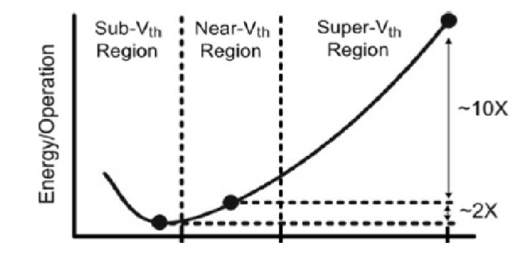
\includegraphics[width=\linewidth]{img/Pictures/Energy_comparison.png}
	\centering
	\caption{Sub/Near-threshold operation. Source: \cite{b1}}
	\label{fig:Energy_comparison}
\end{figure}

The major advantage of using the near threshold devices is the decrese in
Near-Threshold designs refer to operating the transistor slightly above the
threshold region.

Dynamic power per operation is given by ($P_{dyn}=fC_LV_{DD}^2$), and increases
quadratically with voltage but static power per operation increases with
decreasing voltage. This is because the static power
is constant and it increases as the time period per operation increasing.
Hence by adding the two we get a relationship as shown in Fig. \ref{fig:Energy_comparison}. Although we see that the sub-threshold operation
has lower energy than the near-threshold, we want to find a balance between
performance and energy per operation and hence we will investigate the
functionality, variability issues and performance challenges of Near-Threshold
design in this paper.

\section{Functional Challenges of Near-Threshold Design}
\label{sec:Func_challenges}

In the past many works have shown that Near-threshold design is easy to implement for ALUs and logic gates. But SRAM and level Shifter have their challenges in operating in the near-threshold region.

\subsection{Level Shifters}

\begin{figure}[htbp]
	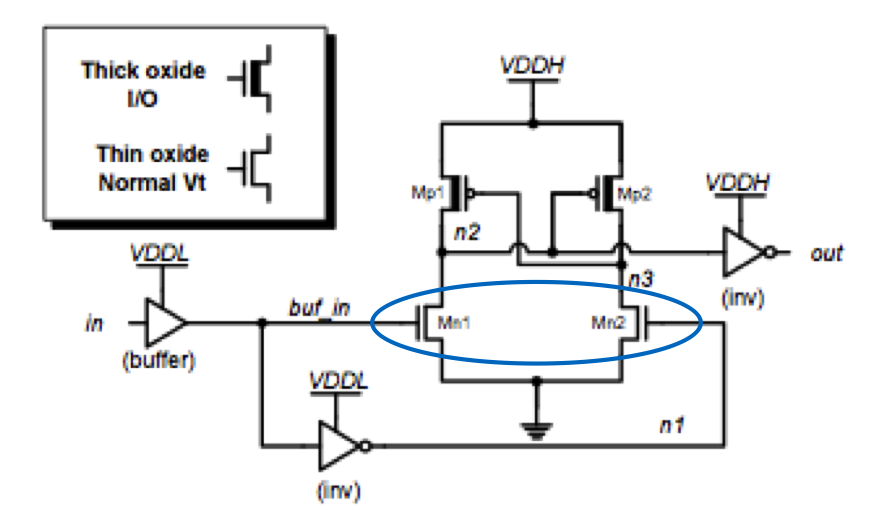
\includegraphics[width=\linewidth]{img/Pictures/Level_shift_weak.png}
	\centering
	\caption{Weak Pull ups Source: \cite{b3}}
	\label{fig:Weak_Pull_ups}
\end{figure}

In the near-threshold operation the pull down network as shown in the Fig. \ref{fig:Weak_Pull_ups} is weaker than the pull up network and consequently the the level shifter cant pull down to ground.

The issue of converting a near-threshold voltage to a super-threshold voltage
therefore needs complex circuitry which is not only low power in nature but
also scales in performance with voltage. 

\begin{figure}[htbp]
	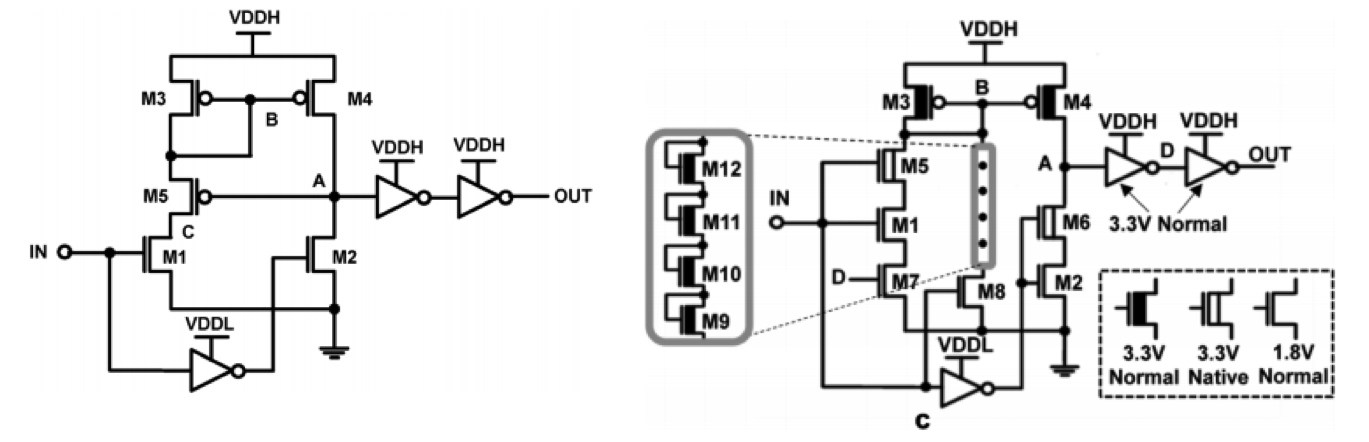
\includegraphics[width=\linewidth]{img/Pictures/Level_shifter_solution.png}
	\centering
	\caption{Weak Pull ups Source: \cite{b6}}
	\label{fig:Level_shifter_solution}
\end{figure}

In \cite{b4}\cite{b5}\cite{b6}, current mirrors based design is suggested which provides performance scalablity
and high energy efficiency as shown in Fig. \ref{fig:Level_shifter_solution}.

\subsection{SRAM Design Challenges}
SRAM prefers small transistors for increased density but

\section{Performance Improvement for Near-Threshold Devices} \label{sec:Perf_challenges}

\subsection{Near-Threshold Device Sizing}
\subsection{Wide Dynamic Voltage Scaling}
\subsection{Parallel Processing}

\section{Manufacturing Variabilty Challenges} \label{sec:Variablity}

\subsection{Library Pruning}
\subsection{Pipeline Optimization}

\section{Architectural Level Power Reduction Techniques} \label{sec:Case_Study}
For high performance embedded devices we need to consider architectural design
changes to maintain the performance. The Application Processor(AP) is the most
power consuming component in the design. In order to reduce the power consumption as
much as possible we need to wake up the AP only when its absolutely necessary.
Given that the peak workload on most mobile embedded devices is often
periodic interrupts or user requests we can utilise this to offload the
AP of servicing these routines.

This is illustrated with the help of a case study to show the advantages of
using an Ultra Low Power Offload Co-processor(OCP), which could be one of the
processors incorporating all the circuit level design techniques described in the earlier sections.

\subsection{Case Study: GPS}

GPS is chosen for our case study as it usually samples at 1Hz and is a periodic
event. Research has shown that GPS can consume upto 95\% of the total power
consumption of the mobile device \cite{b7}.

The system we are considering here is a typical ARM11 micro-processor which is
commonly found in most mobile phones these days. Fig. \ref{fig:Power_profile_ARM11} shows that intially the CPU is in sleep mode
consuming 20mW before the interrupt occurs. The interrupt is excuted in 2ms (at
1000mW) and then cant drop straight away to sleep mode, instead it must operate
at a lower frequency consuming 650mW for 100ms. It drops into another mode at
400mW for another 100ms. Only after excuting in all these intermediate modes
does the CPU go back into deep sleep. Therefore although the interrupt only
takes 2ms to execute the application processor remains active for over 200ms
consuming 60mJ of energy.

\begin{figure}[htbp]
	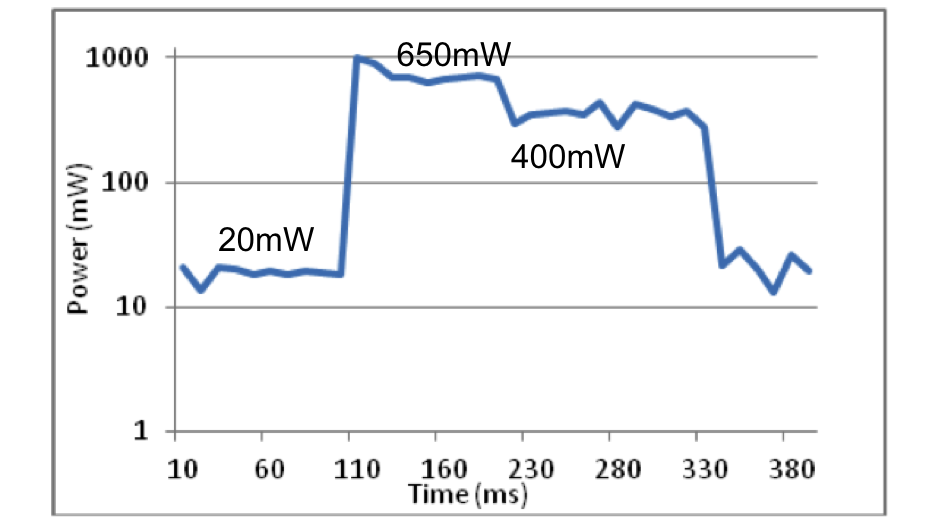
\includegraphics[width=\linewidth]{img/Pictures/Power_profile_ARM11.png}
	\centering
    \caption{Power Profile when a GPS interrupt occurs for an ARM11 CPU: \cite{b2}}
    \label{fig:Power_profile_ARM11}
\end{figure}

An alternative SoC design with a OCP is shown in Fig. \ref{fig:AP}. In our case study the Application Processor is an ARM11 CPU and the OCP is a MIPS32 4KS.

\begin{figure}[htbp]
	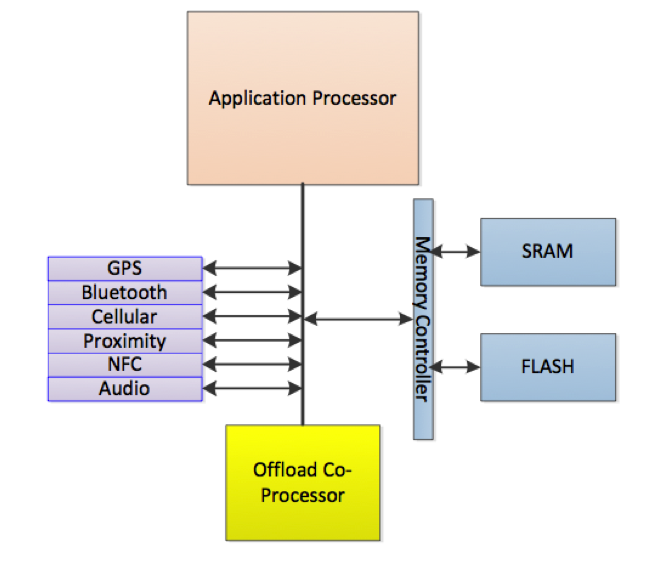
\includegraphics[width=\linewidth]{img/Pictures/AP.png}
	\centering
    \caption{SoC Design with Offload Co-Processor(OCP): \cite{b2}}
    \label{fig:AP}
\end{figure}

\subsection{Considerations for OCP Design}
\subsubsection{Different ISA}
\subsubsection{Interrupt Overheads}
\subsubsection{Interrupt Overflow}
\subsubsection{Hardware Acceleration}

\section{Conclusion}
Circuit design techniques are required to tackle the major challenges of the
near-threshold processor design. Architectural design techniques are required
to add additional power and energy saving. We have demonstrated from the OCP
based SoC design that the battery life can be extended by 3.5 times by adapting
the hybrid approach.

\begin{thebibliography}{00}
\bibitem{b1} J.Zhou, T.H.Kim and Y.Lian, ``Near-threshold processor design techniques for power-constrained 
computing devices,'' 2017 IEEE 12th International Conference on ASIC (ASICON), Guiyang, China, 2017, pp.920-923
\bibitem{b2} J. Tang, C. Liu, Y. L. Chou and S. Liu, ``OCP: Offload Co-Processor
for energy efficiency in embedded mobile systems,'' 2013 IEEE 24th International Conference on Application-Specific 
Systems, Architectures and Processors, Washington, DC, 2013, pp. 107-110
\bibitem{b3} Y. S. Lin, et al., ``Single stage static level shifter designfor subthreshold to I/O voltage conversion,in Proc. ACM/IEEE Int. Symp. Low Power Electron. Design (ISLPED), Aug. 1113, 2008, pp.197200
\bibitem{b4} S. Lutkemeier, et al., ``A subthreshold to above-threshold level shifter comprising a wilson current mirror,'' IEEE Trans. Circuits Syst. II, Exp. Briefs, vol. 57, no. 9, pp. 721724, Sep. 2010
\bibitem{b5} Y. Osaki, et al., ``A low-power level shifter with logic error correction for extremely low-voltage digital CMOS LSIs,'' IEEE J. Solid-State Circuits, vol. 47, no. 7, pp.17761783, Jul. 2012
\bibitem{b6} J. Zhou, et al., ``An Ultra-Low Voltage Level Shifter Using Revised Wilson Current Mirror for Fast and Energy-Efficient Wide-Range Voltage Conversion from Sub-Threshold to I/O Voltage,'' Circuits and Systems I: Regular Papers, IEEE Transactions on , vol.62, no.3, pp.697,706, March 2015
\bibitem{b7} N. Priyantha, D. Lymberopoulos, J. Liu, ``EERS: Energy Efficient Responsive Sleeping on Mobile Phones, in Proceedsings of the International Workshop on Sensing for App Phones'', November, 2010
\end{thebibliography}
\end{document}
